% Options for packages loaded elsewhere
\PassOptionsToPackage{unicode}{hyperref}
\PassOptionsToPackage{hyphens}{url}
\PassOptionsToPackage{dvipsnames,svgnames,x11names}{xcolor}
%
\documentclass[
  letterpaper,
  DIV=11,
  numbers=noendperiod]{scrreprt}

\usepackage{amsmath,amssymb}
\usepackage{lmodern}
\usepackage{iftex}
\ifPDFTeX
  \usepackage[T1]{fontenc}
  \usepackage[utf8]{inputenc}
  \usepackage{textcomp} % provide euro and other symbols
\else % if luatex or xetex
  \usepackage{unicode-math}
  \defaultfontfeatures{Scale=MatchLowercase}
  \defaultfontfeatures[\rmfamily]{Ligatures=TeX,Scale=1}
\fi
% Use upquote if available, for straight quotes in verbatim environments
\IfFileExists{upquote.sty}{\usepackage{upquote}}{}
\IfFileExists{microtype.sty}{% use microtype if available
  \usepackage[]{microtype}
  \UseMicrotypeSet[protrusion]{basicmath} % disable protrusion for tt fonts
}{}
\makeatletter
\@ifundefined{KOMAClassName}{% if non-KOMA class
  \IfFileExists{parskip.sty}{%
    \usepackage{parskip}
  }{% else
    \setlength{\parindent}{0pt}
    \setlength{\parskip}{6pt plus 2pt minus 1pt}}
}{% if KOMA class
  \KOMAoptions{parskip=half}}
\makeatother
\usepackage{xcolor}
\setlength{\emergencystretch}{3em} % prevent overfull lines
\setcounter{secnumdepth}{5}
% Make \paragraph and \subparagraph free-standing
\ifx\paragraph\undefined\else
  \let\oldparagraph\paragraph
  \renewcommand{\paragraph}[1]{\oldparagraph{#1}\mbox{}}
\fi
\ifx\subparagraph\undefined\else
  \let\oldsubparagraph\subparagraph
  \renewcommand{\subparagraph}[1]{\oldsubparagraph{#1}\mbox{}}
\fi


\providecommand{\tightlist}{%
  \setlength{\itemsep}{0pt}\setlength{\parskip}{0pt}}\usepackage{longtable,booktabs,array}
\usepackage{calc} % for calculating minipage widths
% Correct order of tables after \paragraph or \subparagraph
\usepackage{etoolbox}
\makeatletter
\patchcmd\longtable{\par}{\if@noskipsec\mbox{}\fi\par}{}{}
\makeatother
% Allow footnotes in longtable head/foot
\IfFileExists{footnotehyper.sty}{\usepackage{footnotehyper}}{\usepackage{footnote}}
\makesavenoteenv{longtable}
\usepackage{graphicx}
\makeatletter
\def\maxwidth{\ifdim\Gin@nat@width>\linewidth\linewidth\else\Gin@nat@width\fi}
\def\maxheight{\ifdim\Gin@nat@height>\textheight\textheight\else\Gin@nat@height\fi}
\makeatother
% Scale images if necessary, so that they will not overflow the page
% margins by default, and it is still possible to overwrite the defaults
% using explicit options in \includegraphics[width, height, ...]{}
\setkeys{Gin}{width=\maxwidth,height=\maxheight,keepaspectratio}
% Set default figure placement to htbp
\makeatletter
\def\fps@figure{htbp}
\makeatother

\KOMAoption{captions}{tableheading}
\makeatletter
\makeatother
\makeatletter
\@ifpackageloaded{bookmark}{}{\usepackage{bookmark}}
\makeatother
\makeatletter
\@ifpackageloaded{caption}{}{\usepackage{caption}}
\AtBeginDocument{%
\ifdefined\contentsname
  \renewcommand*\contentsname{Table of contents}
\else
  \newcommand\contentsname{Table of contents}
\fi
\ifdefined\listfigurename
  \renewcommand*\listfigurename{List of Figures}
\else
  \newcommand\listfigurename{List of Figures}
\fi
\ifdefined\listtablename
  \renewcommand*\listtablename{List of Tables}
\else
  \newcommand\listtablename{List of Tables}
\fi
\ifdefined\figurename
  \renewcommand*\figurename{Figure}
\else
  \newcommand\figurename{Figure}
\fi
\ifdefined\tablename
  \renewcommand*\tablename{Table}
\else
  \newcommand\tablename{Table}
\fi
}
\@ifpackageloaded{float}{}{\usepackage{float}}
\floatstyle{ruled}
\@ifundefined{c@chapter}{\newfloat{codelisting}{h}{lop}}{\newfloat{codelisting}{h}{lop}[chapter]}
\floatname{codelisting}{Listing}
\newcommand*\listoflistings{\listof{codelisting}{List of Listings}}
\makeatother
\makeatletter
\@ifpackageloaded{caption}{}{\usepackage{caption}}
\@ifpackageloaded{subcaption}{}{\usepackage{subcaption}}
\makeatother
\makeatletter
\@ifpackageloaded{tcolorbox}{}{\usepackage[many]{tcolorbox}}
\makeatother
\makeatletter
\@ifundefined{shadecolor}{\definecolor{shadecolor}{rgb}{.97, .97, .97}}
\makeatother
\makeatletter
\makeatother
\ifLuaTeX
  \usepackage{selnolig}  % disable illegal ligatures
\fi
\IfFileExists{bookmark.sty}{\usepackage{bookmark}}{\usepackage{hyperref}}
\IfFileExists{xurl.sty}{\usepackage{xurl}}{} % add URL line breaks if available
\urlstyle{same} % disable monospaced font for URLs
\hypersetup{
  pdftitle={IPCC Reports and City Climate Change Plans: Proof of concept prototype - Open Climate Reader},
  pdfauthor={FSCI Hackathon Team},
  colorlinks=true,
  linkcolor={blue},
  filecolor={Maroon},
  citecolor={Blue},
  urlcolor={Blue},
  pdfcreator={LaTeX via pandoc}}

\title{IPCC Reports and City Climate Change Plans: Proof of concept
prototype - Open Climate Reader}
\author{FSCI Hackathon Team}
\date{8/4/23}

\begin{document}
\maketitle
\ifdefined\Shaded\renewenvironment{Shaded}{\begin{tcolorbox}[interior hidden, borderline west={3pt}{0pt}{shadecolor}, boxrule=0pt, breakable, enhanced, sharp corners, frame hidden]}{\end{tcolorbox}}\fi

\renewcommand*\contentsname{Table of contents}
{
\hypersetup{linkcolor=}
\setcounter{tocdepth}{2}
\tableofcontents
}
\bookmarksetup{startatroot}

\hypertarget{about-the-prototype}{%
\chapter{About the prototype}\label{about-the-prototype}}

The prototype is a tool for creating `Readers' made from collated
content from IPCC reports. Users can search IPCC Reports, select the
content relevant to their questions and create a reader to share with
others.

The prototype shows answers from IPCC Reports to five FAQ questions
asked about City Climate Plans - outputted as a multi-format Reader -
DOCX, PDF, E-Book, and as sources - all referenced to the orginal
content.

Use case: Climate plan authors need to find IPCC Report recommendations,
sections, visualisations, and external references and use these in their
own city climate plans as well as to distribute the content to their
community for the purpose of making them democratically ---
understandable, accountable, and transparent.

\href{workflow.html}{Read about} the next steps, workflows, and
technologies.

\begin{itemize}
\tightlist
\item
  Next prototype \#2: Automate Reader creation
\item
  Next prototype \#3: AI assisted authoring
\end{itemize}

semanticClimate is looking for support for the protoytpe rounds -
contact semanticClimate on the
\href{https://github.com/petermr/semanticClimate/discussions/32}{GitHub
discussion thread}.

The prototype was made during the semanticClimate hackathon held at the
FORCE11 Scholarly Communications Institute (FSCI) - 2023 Summer School -
July 31 - August 4 2023.

\hypertarget{prototype-questions}{%
\subsection{Prototype questions}\label{prototype-questions}}

Hackathon participants created five questions that are common to City
Climate Plans.

Ahead of technically automating the search the \textbf{mock-up prototype
Reader} shows the types of examples search results that could be
collates.

\hypertarget{questions}{%
\subsubsection{Questions}\label{questions}}

\begin{itemize}
\tightlist
\item
  Q1. What measures can be taken by urban centers to mitigate and cut
  down on their emissions?
\item
  Q2. What role do renewable energy sources play in city climate plans?
\item
  Q3. How can cities promote sustainable transportation options in their
  climate action plans?
\item
  Q4. What strategies do cities employ to adapt to the impacts of
  climate change?
\item
  Q5. What are some successful examples of cities implementing effective
  climate action plans?
\end{itemize}

\hypertarget{background}{%
\subsection{Background}\label{background}}

The IPCC Reports are the source for the most important scientific
knowledge on climate change.

City climate plans are important tools to help mitigate the impacts of
climate change.

Currently IPCC reports are not supported by search services that allow
for granular indexing. The semanticClimate research project uses Linked
Open Data (LOD) and Wikidata / Wikibase technologies to enable better
visibility for the IPCC Report contents.

\hypertarget{links}{%
\subsection{Links}\label{links}}

\begin{itemize}
\tightlist
\item
  semanticClimate project
\item
  About the hackathon
\item
  More about the City Climate Plan Prototype
\item
  FSCI Summer School 2023
\end{itemize}

\hypertarget{credits}{%
\subsection{Credits}\label{credits}}

\begin{itemize}
\tightlist
\item
  See
  \href{https://github.com/semanticClimate/city-climate-plans-notebook/blob/main/README.md}{README.md}
\end{itemize}

\bookmarksetup{startatroot}

\hypertarget{q1.-mitigation-cutting-emmisions}{%
\chapter{Q1. Mitigation \& Cutting
Emmisions?}\label{q1.-mitigation-cutting-emmisions}}

\hypertarget{question-what-measures-can-be-taken-by-urban-centers-to-mitigate-and-cut-down-on-their-emissions}{%
\section{Question: What measures can be taken by urban centers to
mitigate and cut down on their
emissions?}\label{question-what-measures-can-be-taken-by-urban-centers-to-mitigate-and-cut-down-on-their-emissions}}

\hypertarget{query-result-climate-change-2022-mitigation-of-climate-change.-chapter-8-urban-systems-and-other-settlements}{%
\section{Query result: Climate Change 2022: Mitigation of Climate
Change. Chapter 8 : Urban Systems and Other
Settlements}\label{query-result-climate-change-2022-mitigation-of-climate-change.-chapter-8-urban-systems-and-other-settlements}}

Chapter 8 Urban Systems and Other Settlements. In IPCC, 2022: Climate
Change 2022: Mitigation of Climate Change. Contribution of Working Group
III to the 6th Assessment Report of the IPCC

URL: \url{https://www.ipcc.ch/report/ar6/wg3/}

\emph{This chapter should be cited as : Lwasa, S., K.C. Seto, X. Bai, H.
Blanco, K.R. Gurney, Ş. Kılkış, O. Lucon, J. Murakami, J. Pan, A.
Sharifi, Y. Yamagata, 2022: Urban systems and other settlements. In
IPCC, 2022: Climate Change 2022: Mitigation of Climate Change.
Contribution of Working Group III to the Sixth Assessment Report of the
Intergovernmental Panel on Climate Change {[}P.R. Shukla, J. Skea, R.
Slade, A. Al Khourdajie, R. van Diemen, D. McCollum, M. Pathak, S. Some,
P. Vyas, R. Fradera, M. Belkacemi, A. Hasija, G. Lisboa, S. Luz, J.
Malley, (eds.){]}. Cambridge University Press, Cambridge, UK and New
York, NY, USA.}

\begin{center}\rule{0.5\linewidth}{0.5pt}\end{center}

\hypertarget{content}{%
\section{Content:}\label{content}}

\hypertarget{chapter-08-urban-systems-and-other-settlements}{%
\subsection{Chapter 08 : Urban Systems and Other
Settlements}\label{chapter-08-urban-systems-and-other-settlements}}

\hypertarget{executive-summary}{%
\subsubsection{Executive Summary}\label{executive-summary}}

\textbf{Although urbanisation is a global trend often associated with
increased incomes and higher consumption, the growing concentration of
people and activities is an opportunity to increase resource efficiency
and decarbonise at scale (very high confidence).} The same urbanisation
level can have large variations in per capita urban carbon emissions.
For most regions, per capita urban emissions are lower than per capita
national emissions. \{8.1.4, 8.3.3, 8.4, Box 8.1\}

\textbf{Most future urban population growth will occur in developing
countries, where per capita emissions are currently low but expected to
increase with the construction and use of new infrastructure and the
built environment, and changes in incomes and lifestyles (very high
confidence).} The drivers of urban greenhouse gas (GHG) emissions are
complex and include an interplay of population size, income, state of
urbanisation, and how cities are laid out (i.e.~urban form). How new
cities and towns are designed, constructed, managed, and powered will
lock-in behaviour, lifestyles, and future urban GHG emissions.
Low-emission urbanisation can improve well-being while minimising impact
on GHG emissions, but there is risk that urbanisation can lead to
increased global GHG emissions through increased emissions outside the
city's boundaries. \{8.1.4, 8.3, Box 8.1, 8.4, 8.6\}

\textbf{The urban share of global GHG emissions (including carbon
dioxide (CO2) and methane (CH4)) is substantive and continues to
increase (high confidence).} In 2015, urban emissions were estimated to
be 25 GtCO2-eq (about 62\% of the global share) and in 2020, 29 GtCO2-eq
(67--72\% of the global share).1 About 100 of the highest emitting urban
areas account for approximately 18\% of the global carbon footprint.
\{8.1.6, 8.3.3\}

\textbf{The urban share of regional GHG emissions increased between 2000
and 2015, with much inter-region variation in the magnitude of the
increase (high confidence).} Globally, the urban share of national
emissions increased 6 percentage points, from 56\% in 2000 to 62\% in
2015. For 2000 to 2015, the urban emissions share across AR6 WGIII
regions increased from 28\% to 38\% in Africa, from 46\% to 54\% in Asia
and Pacific, from 62\% to 72\% in Developed Countries, from 57\% to 62\%
in Eastern Europe and West-Central Asia, from 55\% to 66\% in Latin
America and Caribbean, and from 68\% to 69\% in the Middle East.
\{8.1.6, 8.3.3\}

\textbf{Per capita urban GHG emissions increased between 2000 and 2015,
with cities in the Developed Countries region producing nearly seven
times more per capita than the lowest emitting region (medium
confidence).} From 2000 to 2015, global urban GHG emissions per capita
increased from 5.5 to 6.2 tCO2-eq per person (an increase of 11.8\%);
Africa increased from 1.3 to 1.5 tCO2-eq per person (22.6\%); Asia and
Pacific increased from 3.0 to 5.1 tCO2-eq per person (71.7\%); Eastern
Europe and West-Central Asia increased from 6.9 to 9.8 tCO2-eq per
person (40.9\%); Latin America and Caribbean increased from 2.7 to 3.7
tCO2-eq per person (40.4\%); and Middle East increased from 7.4 to 9.6
tCO2-eq per person (30.1\%). Albeit starting from the highest level,
Developed Countries had a decline of 11.4 to 10.7 tCO2-eq per person
(--6.5\%). \{8.3.3\}

\textbf{The global share of future urban GHG emissions is expected to
increase through 2050, with moderate to low mitigation efforts, due to
growth trends in population, urban land expansion, and infrastructure
and service demands, but the extent of the increase depends on the
scenario and the scale and timing of urban mitigation action (medium
confidence).} In modelled scenarios, global consumption-based urban CO2
and CH4 emissions are projected to rise from 29 GtCO2-eq in 2020 to 34
GtCO2-eq in 2050 with moderate mitigation efforts (intermediate GHG
emissions, SSP2--4.5), and up to 40 GtCO2-eq in 2050 with low mitigation
efforts (high GHG emissions, SSP3--7.0).

\textbf{Urban land areas could triple between 2015 and 2050, with
significant implications for future carbon lock-in.} There is a large
range in the forecasts of urban land expansion across scenarios and
models, which highlights an opportunity to shape future urban
development towards low- or net-zero GHG emissions and minimise the loss
of carbon stocks and sequestration in the agriculture, forestry and
other land use (AFOLU) sector due to urban land conversion (medium
confidence). By 2050, urban areas could increase up to 211\% over the
2015 global urban extent, with the median projected increase ranging
from 43\% to 106\%. While the largest absolute amount of new urban land
is forecasted to occur in Asia and Pacific, and in Developed Countries,
the highest rate of urban land growth is projected to occur in Africa,
Eastern Europe and West-Central Asia, and in the Middle East. The
infrastructure that will be constructed concomitant with urban land
expansion will lock-in patterns of energy consumption that will persist
for decades if not generations. Furthermore, given past trends, the
expansion of urban areas is likely to take place on agricultural lands
and forests, with implications for the loss of carbon stocks and
sequestration. \{8.3.1, 8.3.4, 8.4.1, 8.6\}

\textbf{The construction of new, and upgrading of, existing urban
infrastructure through 2030 will result in significant emissions (very
high confidence).} The construction of new and upgrading of existing
urban infrastructure using conventional practices and technologies can
result in significant committed CO2 emissions, ranging from 8.5 GtCO2 to
14 GtCO2 annually up to 2030 and more than double annual resource
requirements for raw materials to about 90 billion tonnes per year by
2050, up from 40 billion tonnes in 2010 (medium evidence, high
agreement). \{8.4.1, 8.6\}

\textbf{Given the dual challenges of rising urban GHG emissions and
future projections of more frequent extreme climate events, there is an
urgent need to integrate urban mitigation and adaptation strategies for
cities to address climate change and withstand its effects (very high
confidence).} Mitigation strategies can enhance resilience against
climate change impacts while contributing to social equity, public
health, and human wellbeing. Urban mitigation actions that facilitate
economic decoupling can have positive impacts on employment and local
economic competitiveness. \{8.2, Cross-Working Group Box 2, 8.4\}

\textbf{Cities can only achieve net-zero GHG emissions through deep
decarbonisation and systemic transformation (very high confidence).}
Three broad mitigation strategies have been found to be effective in
reducing emissions when implemented concurrently: (i) reducing or
changing urban energy and material use towards more sustainable
production and consumption across all sectors, including through compact
and efficient urban forms and supporting infrastructure; (ii)
electrification and switching to net-zero-emissions resources; and (iii)
enhancing carbon uptake and storage in the urban environment (high
evidence, high agreement). Given the regional and global reach of urban
supply chains, cities can achieve net-zero emissions only if emissions
are reduced within and outside of their administrative boundaries.
\{8.1.6, 8.3.4, 8.4, 8.6\}

\textbf{Packages of mitigation policies that implement multiple
urbanscale interventions can have cascading effects across sectors,
reduce GHG emissions outside of a city's administrative boundaries, and
reduce more emissions than the net sum of individual interventions,
particularly if multiple scales of governance are included (high
confidence).} Cities have the ability to implement policy packages
across sectors using an urban systems approach, especially those that
affect key infrastructure based on spatial planning, electrification of
the urban energy system, and urban green and blue infrastructure. The
institutional capacity of cities to develop, coordinate, and integrate
sectoral mitigation strategies within their jurisdiction varies by
context, particularly those related to governance, the regulatory
system, and budgetary control. \{8.4, 8.5, 8.6\}

\textbf{Integrated spatial planning to achieve compact and
resourceefficient urban growth through co-location of higher residential
and job densities, mixed land use, and transit-oriented development
(TOD) could reduce GHG emissions between 23\% and 26\% by 2050 compared
to the business-as-usual scenario (robust evidence, high agreement, very
high confidence).} Compact cities with shortened distances between
housing and jobs, and interventions that support a modal shift away from
private motor vehicles towards walking, cycling, and low-emissions
shared and public transportation, passive energy comfort in buildings,
and urban green infrastructure can deliver significant public health
benefits and have lower GHG emissions. \{8.2, 8.3.4, 8.4, 8.6\}

\textbf{Urban green and blue infrastructure can mitigate climate change
through carbon sequestration, avoided emissions, and reduced energy use
while offering multiple co-benefits (robust evidence, high agreement).}
Urban green and blue infrastructure, including urban forests and street
trees, permeable surfaces, and green roofs3 offer potential to mitigate
climate change directly through sequestering and storing carbon, and
indirectly by inducing a cooling effect that reduces energy demand and
reducing energy use for water treatment. Global urban trees store
approximately 7.4 billion tonnes of carbon, and sequester approximately
217 million tonnes of carbon annually, although urban tree carbon
storage and sequestration are highly dependent on biome. Among the
multiple co-benefits of green and blue infrastructure are reducing the
urban heat island (UHI) effect and heat stress, reducing stormwater
runoff, improving air quality, and improving mental and physical health
of urban dwellers. \{8.2, 8.4.4\}

\textbf{The potential and sequencing of mitigation strategies to reduce
GHG emissions will vary depending on a city's land use, spatial form,
development level, and state of urbanisation i.e., whether it is an
established city with existing infrastructure, a rapidly growing city
with new infrastructure, or an emerging city with infrastructure buildup
(high confidence).} New and emerging cities will have significant
infrastructure development needs to achieve high quality of life, which
can be met through energyefficient infrastructures and services, and
people-centred urban design (high confidence). The long lifespan of
urban infrastructures locks in behaviour and committed emissions. Urban
infrastructures and urban form can enable socio-cultural and lifestyle
changes that can significantly reduce carbon footprints. Rapidly growing
cities can avoid higher future emissions through urban planning to
co-locate jobs and housing to achieve compact urban form, and by
leapfrogging to low-carbon technologies. Established cities will achieve
the largest GHG emissions savings by replacing, repurposing, or
retrofitting the building stock, targeted infilling and densifying, as
well as through modal shift and the electrification of the urban energy
system. New and emerging cities have unparalleled potential to become
low or net-zero GHG emissions while achieving high quality of life by
creating compact, co-located, and walkable urban areas with mixed land
use and transit-oriented design, that also preserve existing green and
blue assets. \{8.2, 8.4, 8.6\}

\textbf{With over 880 million people living in informal settlements,
there are opportunities to harness and enable informal practices and
institutions in cities related to housing, waste, energy, water, and
sanitation to reduce resource use and mitigate climate change (low
evidence, medium agreement).} The upgrading of informal settlements and
inadequate housing to improve resilience and well-being offers a chance
to create a lowcarbon transition. However, there is limited quantifiable
data on these practices and their cumulative impacts on GHG emissions.
\{8.1.4, 8.2.2, Cross-Working Group Box 2, 8.3.2, 8.4, 8.6, 8.7\}

\textbf{Achieving transformational changes in cities for climate change
mitigation and adaptation will require engaging multiple scales of
governance, including governments and non-state actors, and in
connection with substantive financing beyond sectoral approaches (very
high confidence).} Large and complex infrastructure projects for urban
mitigation are often beyond the capacity of local municipality budgets,
jurisdictions, and institutions. Partnerships between cities and
international institutions, national and regional governments,
transnational networks, and local stakeholders play a pivotal role in
mobilising global climate finance resources for a range of
infrastructure projects with lowcarbon emissions and related spatial
planning programmes across key sectors. \{8.4, 8.5\}

\hypertarget{footnotes}{%
\subsection{Footnotes}\label{footnotes}}

1 These estimates are based on consumption-based accounting, including
both direct emissions from within urban areas, and indirect emissions
from outside urban areas related to the production of electricity,
goods, and services consumed in cities. Estimates include all CO2 and
CH4 emission categories except for aviation and marine bunker fuels,
land-use change, forestry, and agriculture. \{8.1, Annex I: Glossary\}

2 These scenarios have been assessed by WGI to correspond to
intermediate, high, and very low GHG emissions.

3 These examples are considered to be a subset of nature-based solutions
or ecosystem-based approaches.

\bookmarksetup{startatroot}

\hypertarget{q2.-renewable-energy}{%
\chapter{Q2. Renewable energy?}\label{q2.-renewable-energy}}

\hypertarget{question-what-role-do-renewable-energy-sources-play-in-city-climate-plans}{%
\section{Question: What role do renewable energy sources play in city
climate
plans?}\label{question-what-role-do-renewable-energy-sources-play-in-city-climate-plans}}

\hypertarget{query-result-box-6.8-100-renewables-in-net-zero-energy-systems-page-675-676}{%
\section{Query result: Box 6.8 \textbar{} 100\% Renewables in Net-zero
Energy Systems (Page
675-676)}\label{query-result-box-6.8-100-renewables-in-net-zero-energy-systems-page-675-676}}

Chapter 6 Energy Systems. In IPCC, 2022: Climate Change 2022: Mitigation
of Climate Change. Contribution of Working Group III to the 6th
Assessment Report of the IPCC

URL: \url{https://www.ipcc.ch/report/ar6/wg3/}

\emph{Cite: Clarke, L., Y.-M. Wei, A. De La Vega Navarro, A. Garg, A.N.
Hahmann, S. Khennas, I.M.L. Azevedo, A. Löschel, A.K. Singh, L. Steg, G.
Strbac, K. Wada, 2022: Energy Systems. In IPCC, 2022: Climate Change
2022: Mitigation of Climate Change. Contribution of Working Group III to
the Sixth Assessment Report of the Intergovernmental Panel on Climate
Change {[}P.R. Shukla, J. Skea, R. Slade, A. Al Khourdajie, R. van
Diemen, D. McCollum, M. Pathak, S. Some, P. Vyas, R. Fradera, M.
Belkacemi, A. Hasija, G. Lisboa, S. Luz, J. Malley, (eds.){]}. Cambridge
University Press, Cambridge, UK and New York, NY, USA. doi:
10.1017/9781009157926.008.}

\begin{center}\rule{0.5\linewidth}{0.5pt}\end{center}

\hypertarget{content-1}{%
\section{Content:}\label{content-1}}

\hypertarget{box-6.8-100-renewables-in-net-zero-energy-systems}{%
\subsection{Box 6.8 \textbar{} 100\% Renewables in Net-zero Energy
Systems}\label{box-6.8-100-renewables-in-net-zero-energy-systems}}

The decreasing cost and increasing performance of renewable energy has
generated interest in the feasibility of providing nearly all energy
services with renewables. Renewable energy includes wind power, solar
power, hydroelectric power, bioenergy, geothermal energy, tidal power,
and ocean power. There are two primary frames around which 100\%
renewable energy systems are discussed: 100\% renewable electricity
systems and 100\% renewable energy systems, considering not only
electricity but all aspects of the energy system.

It is technically feasible to use very high renewable shares (e.g.,
above 75\% of annual regional generation) to meet hourly electricity
demand under a range of conditions, especially when VRE options, notably
wind and solar, are complemented by other resources (high confidence).
There are currently many grids with high renewable shares and large
anticipated roles for VRE sources, in particular wind and solar (Section
6.4), in future low-carbon electricity systems. An increasingly large
set of studies examines the feasibility of high renewable penetration
and economic drivers under different policy, technology, and market
scenarios (Cochran et al.~2014; Deason 2018; Jenkins et al.~2018b;
Bistline et al.~2019; Hansen et al.~2019; Dowling et al.~2020; Blanford
et al.~2021; Denholm et al.~2021). High wind and solar penetration
involves technical and economic challenges due to their unique
characteristics such as spatial and temporal variability, short- and
long-term uncertainty, and non-synchronous generation (Cole et
al.~2017). These challenges become increasingly important as renewable
shares approach 100\% (Sections 6.6.2.2 and 6.4.3).

There are many balancing options in systems with very high renewables
(Milligan et al.~2015; Jenkins et al.~2018b; Mai et al.~2018; Bistline
2021a; Denholm et al.~2021).

\begin{itemize}
\tightlist
\item
  Energy storage. Energy storage technologies like batteries, pumped
  hydro, and hydrogen can provide a range of system services (Balducci
  et al.~2018; Bistline et al.~2020a) (Section 6.4.4). Lithium-ion
  batteries have received attention as costs fall and installations
  increase, but very high renewable shares typically entail either
  dispatchable generation or long-duration storage in addition to
  short-duration options (Jenkins et al.~2018b; Arbabzadeh et al.~2019;
  Schill 2020). Energy storage technologies are part of a broad set of
  options (including synchronous condensers, demand-side measures, and
  even inverter-based technologies themselves) for providing grid
  services (Castillo and Gayme 2014; EPRI 2019a).
\item
  Transmission and trade. To balance differences in resource
  availability, high renewable systems will very likely entail
  investments in transmission capacity (Mai et al.~2014; Macdonald et
  al.~2016; Pleßmann and Blechinger 2017; Zappa et al.~2019) (Section
  6.4.5) and changes in trade (Abrell and Rausch 2016; Bistline et
  al.~2019). These increases will likely be accompanied by expanded
  balancing regions to take advantage of geographical smoothing.
\item
  Dispatchable (`on-demand') generation. Dispatchable generation could
  include flexible fossil units or low-carbon fuels such as hydrogen
  with lower minimum load levels (Denholm et al.~2018; Bistline 2019),
  renewables like hydropower, geothermal, or biomass (Hirth 2016; Hansen
  et al.~2019), or flexible nuclear (Jenkins et al.~2018a). The
  composition depends on costs and other policy goals, though in all
  cases, capacity factors are low for these resources (Mills et
  al.~2020).
\item
  Demand management: Many low-emitting and high-renewables systems also
  utilise increased load flexibility in the forms of energy efficiency,
  demand response, and demand flexibility, utilising newly electrified
  end uses such as electric vehicles to shape demand profiles to better
  match supply (Ameli et al.~2017; Hale 2017; Brown et al.~2018; Imelda
  et al.~2018a; Bistline 2021a). • Sector coupling: Sector coupling
  includes increased end-use electrification and PtX electricity
  conversion pathways, which may entail using electricity to create
  synthetic fuels such as hydrogen (Davis et al.~2018; Ueckerdt et
  al.~2021) (Sections 6.4.3, 6.4., 6.4.5, 6.6.4.3, and 6.6.4.6).
\end{itemize}

Deployment of integration options depends on their relative costs and
value, regulations, and electricity market design. There is considerable
uncertainty about future technology costs, performance, availability,
scalability, and public acceptance (Kondziella and Bruckner 2016;
Bistline et al.~2019). Deploying balanced resources likely requires
operational, market design, and other institutional changes, as well as
technological changes in some cases (Denholm et al.~2021; Cochran et
al.~2014). Mixes will differ based on resources, system size,
flexibility, and whether grids are isolated or interconnected.

Although there are no technical upper bounds on renewable electricity
penetration, the economic value of additional wind and solar capacity
typically decreases as their penetration rises, creating economic
challenges at higher deployment levels (Hirth 2013; Gowrisankaran et
al.~2016; Cole et al.~2021; Denholm et al.~2021; Millstein et al.~2021).
The integration options above, as well as changes to market design, can
mitigate these challenges but likely will not solve them, especially
since these options can exhibit declining value themselves (De Sisternes
et al.~2016; Bistline 2017; Denholm and Mai 2019) and may be complements
or substitutes to each other.

Energy systems that are 100\% renewable (including all parts of the
energy sector, and not only electricity generation) raise a range of
technological, regulatory, market, and operational challenges that make
their competitiveness uncertain (high confidence). These systems require
decarbonising all electricity, using this zero-carbon electricity
broadly, and then utilising zero-carbon energy carriers for all end uses
not served by electricity, for example, air travel, long-distance
transport, and high-temperature process heat. Broader questions emerge
regarding the attractiveness of supplying all energy, and not just
electricity, with renewables (Figure 6.22). Integrated assessment and
energy systems research suggest large roles for renewables, but energy
and electricity shares are far from 100\%, even with stringent emissions
reductions targets and optimistic assumptions about future cost
reductions (Bauer et al.~2018; Bistline et al.~2018; Jenkins et
al.~2018b; Huntington et al.~2020) (Section 6.7.1). Scenarios with 100\%
renewable energy systems are an emerging subset in the decarbonisation
literature, especially at regional levels (Hansen et al.~2019; Denholm
et al.~2021). Many 100\% renewables studies focus more heavily on
electrification for decarbonising end uses, and include less biofuels
and hydrogen than the broader literature on deep decarbonisation (Bauer
et al.~2018a). These studies typically assume a constrained set of
available technologies to demonstrate the technical feasibility of very
high renewable systems and do not optimise to find least-cost,
technology-neutral decarbonisation pathways, and many 100\% renewables
studies focus on the electricity sector or a limited number of sectors
(Jenkins et al.~2018a; Hansen et al.~2019). In addition to renewables,
studies broadly agree that including additional lowcarbon options --
including not only low-carbon electricity but also targeted use of
fossil fuels with and without CCS (Section 6.6.2.1) and alternative
fuels for sectors that are difficult to electrify (Section 6.6.2.4) --
can lower the cost of decarbonisation, even with very high shares of
renewables (Figure 6.22). However, there is disagreement about the
magnitude of cost savings from larger portfolios, which depend on
context- and scenario-specific assumptions about technologies, markets,
and policies.

\bookmarksetup{startatroot}

\hypertarget{q3.-sustainable-transport-options}{%
\chapter{Q3. Sustainable Transport
Options?}\label{q3.-sustainable-transport-options}}

\hypertarget{question-how-can-cities-promote-sustainable-transportation-options-in-their-climate-action-plans}{%
\section{Question: How can cities promote sustainable transportation
options in their climate action
plans?}\label{question-how-can-cities-promote-sustainable-transportation-options-in-their-climate-action-plans}}

\hypertarget{query-result-10.7.4-transport-modes-trajectories-page-1104-1106}{%
\section{Query result: 10.7.4 Transport Modes Trajectories (Page
1104-1106)}\label{query-result-10.7.4-transport-modes-trajectories-page-1104-1106}}

Chapter 10 Transport. In IPCC, 2022: Climate Change 2022: Mitigation of
Climate Change. Contribution of Working Group III to the 6th Assessment
Report of the IPCC

URL: \url{https://www.ipcc.ch/report/ar6/wg3/}

\emph{Cite: Jaramillo, P., S. Kahn Ribeiro, P. Newman, S. Dhar, O.E.
Diemuodeke, T. Kajino, D.S. Lee, S.B. Nugroho, X. Ou, A. Hammer
Strømman, J. Whitehead, 2022: Transport. In IPCC, 2022: Climate Change
2022: Mitigation of Climate Change. Contribution of Working Group III to
the Sixth Assessment Report of the Intergovernmental Panel on Climate
Change {[}P.R. Shukla, J. Skea, R. Slade, A. Al Khourdajie, R. van
Diemen, D. McCollum, M. Pathak, S. Some, P. Vyas, R. Fradera, M.
Belkacemi, A. Hasija, G. Lisboa, S. Luz, J. Malley, (eds.){]}. Cambridge
University Press, Cambridge, UK and New York, NY, USA. doi:
10.1017/9781009157926.012}

\begin{center}\rule{0.5\linewidth}{0.5pt}\end{center}

\hypertarget{content-2}{%
\section{Content:}\label{content-2}}

\hypertarget{transport-modes-trajectories}{%
\subsection{10.7.4 Transport Modes
Trajectories}\label{transport-modes-trajectories}}

\begin{figure}

{\centering 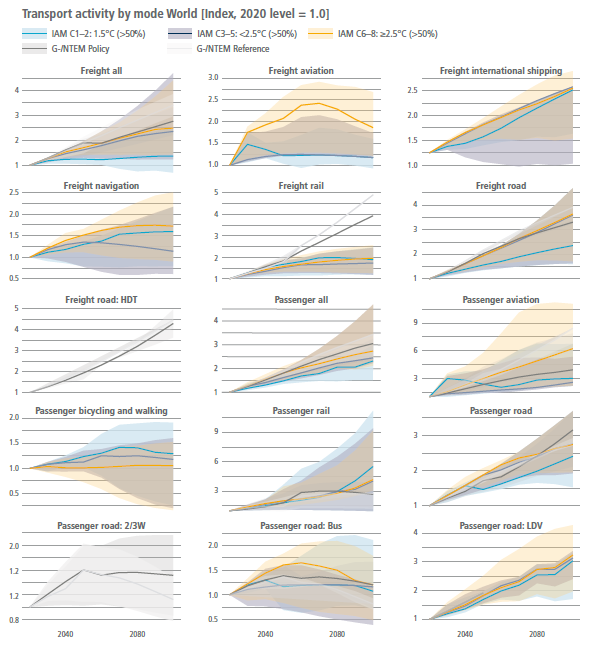
\includegraphics{./images/Fig-10.19.PNG}

}

\caption{\textbf{Figure 10.19 \textbar{} Transport activity trajectories
for passenger and freight across different modes.} Global passenger
(billion pkm per year) and freight (billion tkm per year) demand
projections relative to a modelled year 2020 index. Results for IAM are
for selected stabilisation temperatures by 2100. Also included are
global transport models Reference and Policy scenarios. Data from the
AR6 scenario database. Trajectories span the 5th to 95th percentiles
across models, with a solid line indicating the median value across
models.}

\end{figure}

Globally over the last century, shares of faster transport modes have
generally increased with increasing passenger travel demand (Schäfer
2017; Schafer and Victor 2000). For short- to medium-distance travel,
private cars have displaced public transit, particularly in OECD
countries, due to a variety of factors, including faster travel times in
many circumstances (Liao et al.~2020); consumers increasingly valuing
time and convenience with GDP growth; and broader transport policies,
such as provision of road versus public transit infrastructure (Mattioli
et al.~2020). For long-distance travel, travel via aviation for leisure
and business has increased (Lee et al.~2021). These trends do not hold
in all countries and cities, as many now have rail transit that is
faster than driving (Newman et al.~2015). For instance, public transport
demand rose from 1990 through to 2016 in France, Denmark, and Finland
(eurostat 2019). In general, smaller and denser countries and cities
with higher or increasing urbanisation rates tend to have greater
success in increasing public transport share. However, other factors,
like privatisation of public transit (Bayliss and Mattioli 2018) and
urban form (ITF 2021), also play a role. Different transport modes can
provide passenger and freight services, affecting the emissions
trajectories for the sector.

Figure 10.19 shows activity trajectories for freight and passenger
transport through 2100 relative to a modelled year 2020 across different
modes, based on the AR6 database for IAMs and global transport models.
Globally, climate scenarios from IAMs, and policy and reference
scenarios from global transport models, indicate increasing demand for
freight and passenger transport via most modes through 2100 (Yeh et
al.~2017; Mulholland et al.~2018; Zhang et al. 2018; Khalili et
al.~2019). Road passenger transport exhibits a similar increase (roughly
tripling) through 2100 across scenarios. For road passenger transport,
scenarios that limit or return warming to 1.5°C during the 21st century
(C1--C2) have a smaller increase from modelled 2020 levels (median
increase of 2.4 times modelled 2020 levels) than do scenarios with
higher warming levels (C3--C8) (median increase of 2.7--2.8 times
modelled 2020 levels). There are similar patterns for passenger road
transport via light-duty vehicle, for which median increases from
modelled 2020 levels are smaller for C1--C2 (3 times larger) than for
C3--C5 (3.1 times larger) or C6--C7 (3.2 times larger). Passenger
transport via aviation exhibits a 2.2 times median increase relative to
modelled 2020 levels under C1--C2 and C3--C5 scenarios but exhibits a
6.2 times increase under C6--C8. The only passenger travel mode that
exhibits a decline in its median value through 2100 according to IAMs is
walking/bicycling, in C3-- C5 and C6--C8 scenarios. However, in C1--C2
scenarios, walking/ bicycling increases by 1.4 times relative to
modelled 2020 levels. At the 5th percentile of IAM solutions (lower edge
of bands in Figure 10.19), buses and walking/bicycling for passenger
travel both exhibit significant declines.

For freight, Figure 10.19 shows that the largest growth occurs in
transport via road (Mulholland et al.~2018). By 2100, global transport
models suggest a roughly four-fold increase in median-heavy-duty
trucking levels relative to modelled 2020 levels, while IAMs suggest a
two- to four-fold increase in freight transport by road by 2100.
Notably, the 95th percentile of IAM solutions see road transport by up
to 4.7 times through 2100 relative to modelled 2020 levels, regardless
of warming level. Other freight transport modes -- aviation,
international shipping, navigation, and railways -- exhibit less growth
than road transport. In scenarios that limit or return warming to 1.5°C
(\textgreater50\%) during the 21st century (C1--C2), navigation and rail
transport remain largely unchanged and international shipping roughly
doubles by 2100. Scenarios with higher warming (i.e., moving from C1--C2
to C6--C8) generally lead to more freight by rail and less freight by
international shipping.

Relative to global trajectories, upper-income regions -- including North
America, Europe, and the Pacific OECD -- generally see less growth in
passenger road via light-duty vehicle and passenger aviation, given more
saturated demand for both. Other regions like China exhibit similar
modal trends as the global average, whereas regions such as the African
continent and Indian subcontinent exhibit significantly larger shifts,
proportionally, in modal transport than the globe. In particular, the
African continent represents the starkest departure from global results.
Freight and passenger transport modes exhibit significantly greater
growth across Africa than globally in all available scenarios. Across
Africa, median freight and passenger transport via road from IAMs
increases by 5 to 16 times and 4 to 28 times, respectively, across
warming levels by 2100 relative to modelled 2020 levels. Even C1 has
considerable growth in Africa via both modes (3 to 16 times increase for
freight and 4 to 29 times increase for passenger travel at 5th and 95th
percentiles of IAM solutions by 2100).

As noted in Section 10.2, commonly explored mitigation options related
to mode change include a shift to public transit, shared mobility, and
demand reductions through various means, including improved urban form,
teleconferences that replace passenger travel (Creutzig et al.~2018;
Grubler et al.~2018; Wilson et al.~2019), improved logistics efficiency,
green logistics, and streamlined supply chains for the freight sector
(Mulholland et al.~2018). NDCs often prioritise options like bus
improvements and enhanced mobility that yield pollution, congestion, and
urban development co-benefits, especially in medium- and lower-income
countries (Fulton et al. 2017). Conversely, high-income countries, most
of which have saturated and entrenched private vehicle ownership,
typically focus more on technology options, such as electrification and
fuel efficiency standards (Gota et al.~2016). Available IAM and regional
models are limited in their ability to represent modal shift strategies.
As a result, mode shifts alone do not differentiate climate scenarios.
While this lack of representation is a limitation of the models, it is
unlikely that such interventions would completely negate the increases
in demand the models suggest. Therefore, transport via light-duty
vehicle and aviation, freight transport via road, and other modes will
likely continue to increase through to the end of the century.
Consequently, fuel and carbon efficiency and fuel energy and technology
will probably play crucial roles in differentiating climate scenarios,
as discussed in the following sub-sections.

\bookmarksetup{startatroot}

\hypertarget{q4.-adapting-to-impacts}{%
\chapter{Q4. Adapting to Impacts?}\label{q4.-adapting-to-impacts}}

\hypertarget{question-what-strategies-do-cities-employ-to-adapt-to-the-impacts-of-climate-change}{%
\section{Question: What strategies do cities employ to adapt to the
impacts of climate
change?}\label{question-what-strategies-do-cities-employ-to-adapt-to-the-impacts-of-climate-change}}

\hypertarget{query-result-4.5.3.-cities-settlements-and-infrastructure-page-105-106}{%
\section{Query result: 4.5.3. Cities, Settlements and Infrastructure
(Page
105-106)}\label{query-result-4.5.3.-cities-settlements-and-infrastructure-page-105-106}}

IPCC, 2023: Climate Change 2023: Synthesis Report. Section 4: Near-Term
Responses in a Changing Climate \textgreater{} 4.5 Near-Term Mitigation
and Adaptation Actions \textgreater{} 4.5.3 Cities, Settlements and
Infrastructure

URL: \url{https://www.ipcc.ch/report/ar6/syr/}

\emph{Cite: IPCC, 2023: Climate Change 2023: Synthesis Report.
Contribution of Working Groups I, II and III to the Sixth Assessment
Report of the Intergovernmental Panel on Climate Change {[}Core Writing
Team, H. Lee and J. Romero (eds.){]}. IPCC, Geneva, Switzerland, 184
pp., doi: 10.59327/IPCC/AR6-9789291691647.}

\begin{center}\rule{0.5\linewidth}{0.5pt}\end{center}

\hypertarget{content-3}{%
\section{Content:}\label{content-3}}

\hypertarget{cities-settlements-and-infrastructure}{%
\subsection{4.5.3. Cities, Settlements and
Infrastructure}\label{cities-settlements-and-infrastructure}}

Urban systems are critical for achieving deep emissions reductions and
advancing climate resilient development, particularly when this involves
integrated planning that incorporates physical, natural and social
infrastructure (high confidence). Deep emissions reductions and
integrated adaptation actions are advanced by: integrated, inclusive
land use planning and decision-making; compact urban form by co-locating
jobs and housing; reducing or changing urban energy and material
consumption; electrification in combination with low emissions sources;
improved water and waste management infrastructure; and enhancing carbon
uptake and storage in the urban environment (e.g.~bio-based building
materials, permeable surfaces and urban green and blue infrastructure).
Cities can achieve net zero emissions if emissions are reduced within
and outside of their administrative boundaries through supply chains,
creating beneficial cascading effects across other sectors. (high
confidence) \{WGII SPM C.5.6, WGII SPM D.1.3, WGII SPM D.3; WGIII SPM
C.6, WGIII SPM C.6.2, WGIII TS 5.4, SR1.5 SPM C.2.4\}

Considering climate change impacts and risks (e.g., through climate
services) in the design and planning of urban and rural settlements and
infrastructure is critical for resilience and enhancing human
well-being. Effective mitigation can be advanced at each of the design,
construction, retrofit, use and disposal stages for buildings.
Mitigation interventions for buildings include: at the construction
phase, low-emission construction materials, highly efficient building
envelope and the integration of renewable energy solutions; at the use
phase, highly efficient appliances/equipment, the optimisation of the
use of buildings and their supply with low-emission energy sources; and
at the disposal phase, recycling and re-using construction materials.
Sufficiency155 measures can limit the demand for energy and materials
over the lifecycle of buildings and appliances. (high confidence) \{WGII
SPM C.2.5; WGIII SPM C.7.2\}

Transport-related GHG emissions can be reduced by demand-side options
and low-GHG emissions technologies. Changes in urban form, reallocation
of street space for cycling and walking, digitalisation (e.g.,
teleworking) and programs that encourage changes in consumer behaviour
(e.g.~transport, pricing) can reduce demand for transport services and
support the shift to more energy efficient transport modes (high
confidence). Electric vehicles powered by low-emissions electricity
offer the largest decarbonisation potential for land-based transport, on
a life cycle basis (high confidence). Costs of electrified vehicles are
decreasing and their adoption is accelerating, but they require
continued investments in supporting infrastructure to increase scale of
deployment (high confidence). The environmental footprint of battery
production and growing concerns about critical minerals can be addressed
by material and supply diversification strategies, energy and material
efficiency improvements, and circular material flows (medium
confidence). Advances in battery technologies could facilitate the
electrification of heavy-duty trucks and compliment conventional
electric rail systems (medium confidence). Sustainable biofuels can
offer additional mitigation benefits in land-based transport in the
short and medium term (medium confidence). Sustainable biofuels,
low-emissions hydrogen, and derivatives (including synthetic fuels) can
support mitigation of CO2 emissions from shipping, aviation, and
heavy-duty land transport but require production process improvements
and cost reductions (medium confidence). Key infrastructure systems
including sanitation, water, health, transport, communications and
energy will be increasingly vulnerable if design standards do not
account for changing climate conditions (high confidence). \{WGII SPM
B.2.5; WGIII SPM C.6.2, WGIII SPM C.8, WGIII SPM C.8.1, WGIII SPM C.8.2,
WGIII SPM C.10.2, WGIII SPM C.10.3, WGIII SPM C.10.4\}

Green/natural and blue infrastructure such as urban forestry, green
roofs, ponds and lakes, and river restoration can mitigate climate
change through carbon uptake and storage, avoided emissions, and reduced
energy use while reducing risk from extreme events such as heatwaves,
heavy precipitation and droughts, and advancing co-benefits for health,
well-being and livelihoods (medium confidence). Urban greening can
provide local cooling (very high confidence). Combining green/natural
and grey/physical infrastructure adaptation responses has potential to
reduce adaptation costs and contribute to flood control, sanitation,
water resources management, landslide prevention and coastal protection
(medium confidence). Globally, more financing is directed at
grey/physical infrastructure than green/natural infrastructure and
social infrastructure (medium confidence), and there is limited evidence
of investment in informal settlements (medium to high confidence). The
greatest gains in well-being in urban areas can be achieved by
prioritising finance to reduce climate risk for low-income and
marginalised communities including people living in informal settlements
(high confidence). \{WGII SPM C.2.5, WGII SPM C.2.6, WGII SPM C.2.7,
WGII SPM D.3.2, WGII TS.E.1.4, WGII Cross-Chapter Box FEAS; WGIII SPM
C.6, WGIII SPM C.6.2, WGIII SPM D.1.3, WGIII SPM D.2.1\}

Responses to ongoing sea level rise and land subsidence in low-lying
coastal cities and settlements and small islands include protection,
accommodation, advance and planned relocation. These responses are more
effective if combined and/or sequenced, planned well ahead, aligned with
sociocultural values and development priorities, and underpinned by
inclusive community engagement processes. (high confidence) \{WGII SPM
C.2.8\}

\bookmarksetup{startatroot}

\hypertarget{q5.-successful-example-plans}{%
\chapter{Q5. Successful example
plans?}\label{q5.-successful-example-plans}}

\hypertarget{question-what-are-some-successful-examples-of-cities-implementing-effective-climate-action-plans}{%
\section{Question: What are some successful examples of cities
implementing effective climate action
plans?}\label{question-what-are-some-successful-examples-of-cities-implementing-effective-climate-action-plans}}

\hypertarget{query-result-box-8.3-coordination-of-fragmented-policymaking-for-low-carbon-urban-development-example-from-shanghai-china-page-913}{%
\section{Query result: Box 8.3: Coordination of Fragmented Policymaking
for Low-carbon Urban Development: Example from Shanghai, China (Page
913)}\label{query-result-box-8.3-coordination-of-fragmented-policymaking-for-low-carbon-urban-development-example-from-shanghai-china-page-913}}

Chapter 8 Urban Systems and Other Settlements. In IPCC, 2022: Climate
Change 2022: Mitigation of Climate Change. Contribution of Working Group
III to the 6th Assessment Report of the IPCC

URL: \url{https://www.ipcc.ch/report/ar6/wg3/}

\emph{Cite: This chapter should be cited as : Lwasa, S., K.C. Seto, X.
Bai, H. Blanco, K.R. Gurney, Ş. Kılkış, O. Lucon, J. Murakami, J. Pan,
A. Sharifi, Y. Yamagata, 2022: Urban systems and other settlements. In
IPCC, 2022: Climate Change 2022: Mitigation of Climate Change.
Contribution of Working Group III to the Sixth Assessment Report of the
Intergovernmental Panel on Climate Change {[}P.R. Shukla, J. Skea, R.
Slade, A. Al Khourdajie, R. van Diemen, D. McCollum, M. Pathak, S. Some,
P. Vyas, R. Fradera, M. Belkacemi, A. Hasija, G. Lisboa, S. Luz, J.
Malley, (eds.){]}. Cambridge University Press, Cambridge, UK and New
York, NY, USA.}

\begin{center}\rule{0.5\linewidth}{0.5pt}\end{center}

\hypertarget{content-4}{%
\section{Content:}\label{content-4}}

\hypertarget{chapter-08-urban-systems-and-other-settlements-1}{%
\subsection{Chapter 08 : Urban Systems and Other
Settlements}\label{chapter-08-urban-systems-and-other-settlements-1}}

\hypertarget{box-8.3-coordination-of-fragmented-policymaking-for-low-carbon-urban-development-example-from-shanghai-china}{%
\subsubsection{Box 8.3: Coordination of Fragmented Policymaking for
Low-carbon Urban Development: Example from Shanghai,
China}\label{box-8.3-coordination-of-fragmented-policymaking-for-low-carbon-urban-development-example-from-shanghai-china}}

As a growing megacity in the Global South, Shanghai represents the
challenge of becoming low carbon despite its economic growth and
population size (Chen et al.~2017). Shanghai was designated as one of
the pilot low-carbon cities by the central government. The city utilised
a coordination mechanism for joining fragmented policymaking across the
city's economy, energy, and environment. The coordination mechanism was
supported by a direct fund that enabled implementation of cross-sector
policies beyond a singlesector focus across multiple institutions while
increasing capacity for enabling a low-carbon transition for urban
sustainability (Peng and Bai 2020).

\textbf{Implementation and governance process}

In Shanghai, coordination between the central and local governments had
an instrumental role for encouraging low-carbon policy experimentation.
Using a nested governance framework, the central government provided
target setting and performance evaluation while the local government
initiated pilot projects for low-carbon development. The policy
practices in Shanghai surpassed the topdown targets and annual reporting
of GHG emissions, including carbon labelling standards at the local
level, pilot programme for transitioning sub-urban areas, and the
engagement of public utilities (Peng and Bai 2018).

\textbf{Towards low-carbon urban development}

New policy measures in Shanghai were built upon a series of related
policies from earlier, ranging from general energy saving measures to
air pollution reduction. This provided a continuum of policy learning
for implementing low-carbon policy measures. An earlier policy was a
green electricity scheme based on the Jade Electricity Program while the
need for greater public awareness was one aspect requiring further
attention in policy design (Baeumler et al.~2012), supporting
policy-learning for policies later on. The key point here is that
low-carbon policies were built on and learned from earlier policies with
similar goals.

\textbf{Outcomes and impacts of the policy mix}

Trends during 1998 and 2015 indicate that energy intensity decreased
from about 130 tonnes per million RMB to about 45 tonnes per million RMB
and carbon intensity decreased from about 0.35 Mt per billion RMB to
0.10 Mt per billion RMB (Peng and Bai 2018). These impacts on energy and
carbon intensities represent progress, while challenges remain. Among
the challenges are the need for investment in low-carbon technology and
increases in urban carbon sinks (Yang and Li 2018) while cross-sector
interaction and complexity are increasing.

\bookmarksetup{startatroot}

\hypertarget{prototype-next-steps-workflows}{%
\chapter{Prototype Next Steps \&
Workflows}\label{prototype-next-steps-workflows}}

\begin{figure}

{\centering 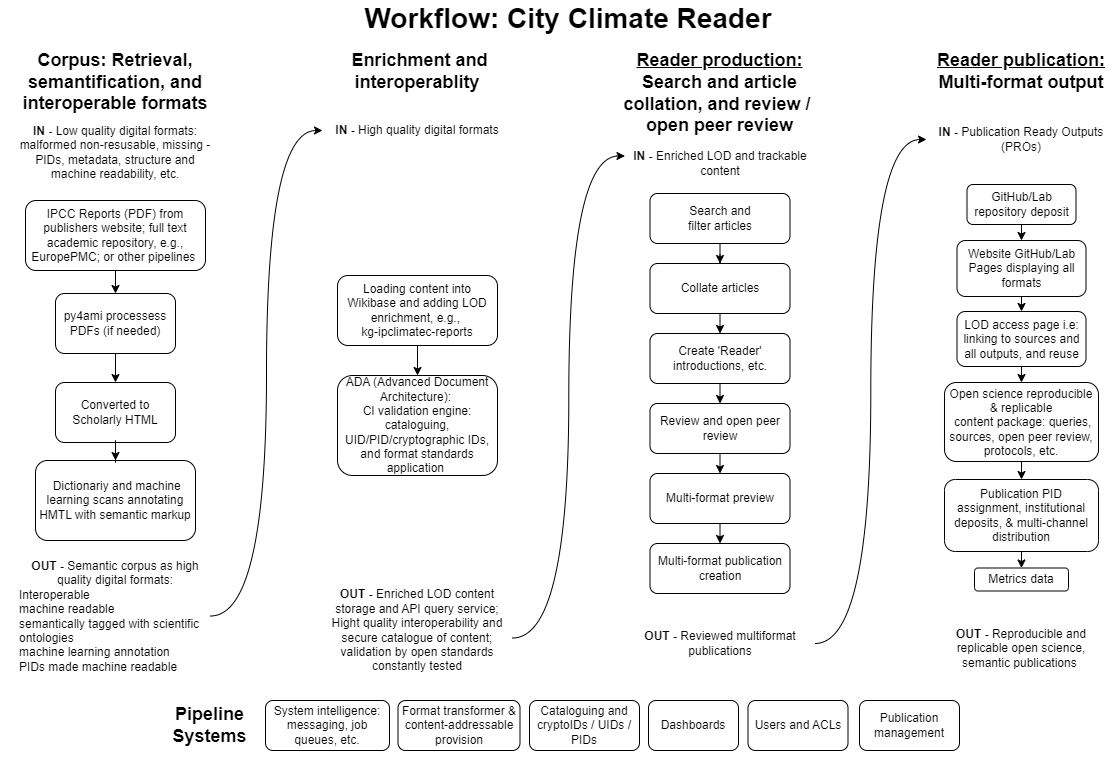
\includegraphics{./workflows/city climate reader workflow v1.drawio.png}

}

\caption{Workflow: City Climate Reader}

\end{figure}

\begin{figure}

{\centering 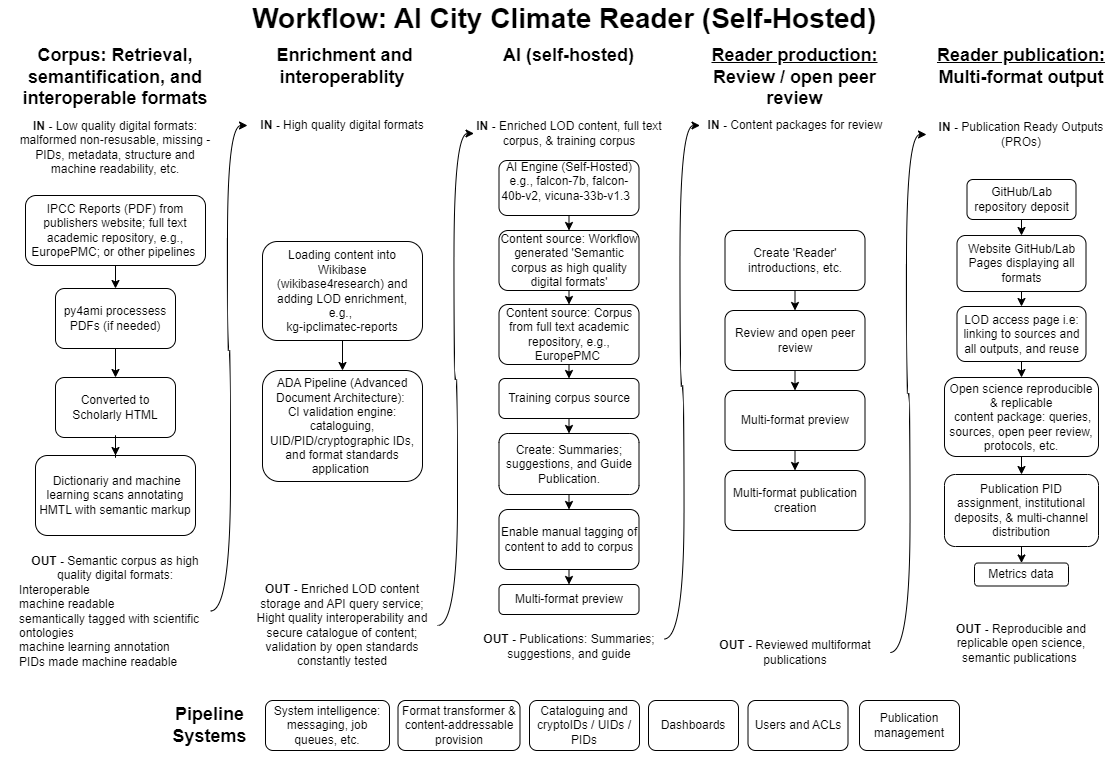
\includegraphics{./workflows/AI city climate reader workflow v1.drawio.png}

}

\caption{Workflow: AI City Climate Reader}

\end{figure}

See diagrams here:
\url{https://github.com/semanticClimate/city-climate-plans-notebook/tree/main/workflows}

\hypertarget{next-steps}{%
\section{Next steps?}\label{next-steps}}

If you're interested in helping out on the next round of prototyping by
volunteering or contributing resources check out the semanticClimate
\href{https://github.com/petermr/semanticClimate/discussions/32}{discussion}
and \href{https://github.com/orgs/semanticClimate/projects/3}{project
tasks} on GitHub.

\hypertarget{a-working-prototype-for-climate-reader}{%
\subsection{A working prototype for Climate
Reader}\label{a-working-prototype-for-climate-reader}}

The round of work from the hackathon allowed the team to see the gaps in
the system and what would need to be put in place to have a working
prototype --- meaning we now have a roadmap. There are four priority
areas to work on for a working prototype: 1. How to smoothly move
contributors' questions into the search and content retrieval process?
2. How to create citation links to sections of the source material which
are only held as PDFs and so can't be targeted on a granular basis?
\href{https://semanticclimate.org/IPCC-Queries/}{Wikibase} has already
been used by semanticClimate and is one route forward for this. 3.
Further automating the conversion of HTML content to Markdown. 4. Adding
a review process to the collated reader content.

\hypertarget{ai-prototype-self-hosted}{%
\subsection{AI prototype (self-hosted)}\label{ai-prototype-self-hosted}}

AI Climate Reader is a proof of concept software prototype that can
query scientific corpora and create `reader' publications combining AI
with added human review. The types of `reader' publications it would
make are: Referenced summaries, suggestions for literature, and guides
on specific topics. The publications would have all the references
collated as full text in the publication. 1. Deposit content in a
Wikibase instance as with the
\href{https://semanticclimate.org/IPCC-Queries/}{AR6 IPCC Report}. New
Wikibase instances are supplied by
\href{https://nfdi4culture.de/services/details/wikibase4research.html}{Wikibase4Research}.
2. Then self-hosted AI would be used to create the publications ---
example AI models are
\href{https://huggingface.co/h2oai/h2ogpt-gm-oasst1-en-2048-falcon-7b-v3}{falcon-7b},
\href{https://huggingface.co/h2oai/h2ogpt-gm-oasst1-en-2048-falcon-40b-v2}{falcon-40b-v2},
\href{https://huggingface.co/lmsys/vicuna-33b-v1.3}{vicuna-33b-v1.3}. 3.
Review and multi-format publishing is then run to create a reproducible
and replicable open science, semantic publication on GitHub/Lab Pages
using the \href{https://github.com/TIBHannover/ADA}{ADA Semantic
Publishing Pipeline} which harnesses Fidus Writer and its Open Journals
System JATS editor plugin.



\end{document}
